
\mychapter{System Modeling \& Theoretical Design}{System Modeling \& Theoretical Design}{}
\label{chap:Overall-System-Design-and-Modeling}

\section{System Architecture}
The proposed hardware architecture of the potentiostat is illustrated in Figure \ref{fig:system_architecture} is divided into high-level software logic and discrete hardware components. The architecture is designed to be modular, allowing for easy integration of various components. The analog front-end serves as the core of the system, providing the necessary tools for electrochemical measurements. The microcontroller manages data acquisition, processing, and communication. The physical user interface allows for local control and user input and control. The three-electrode setup ensures accurate electrochemical measurements, making the system suitable for detecting trace levels of antiretroviral medications in water samples.

The software architecture manages the analytical core and connectivity of the system. It is driven by real-time operating system and features an embedded web server and Wi-Fi capabilities for data extraction and review alongside data storage. The analytical core manages the DPV waveform generation and differential current calculations, while a local GUI and display driver ensure the physical interface is operational without the need for an external smart device.

\begin{figure}[H]
    \centering
    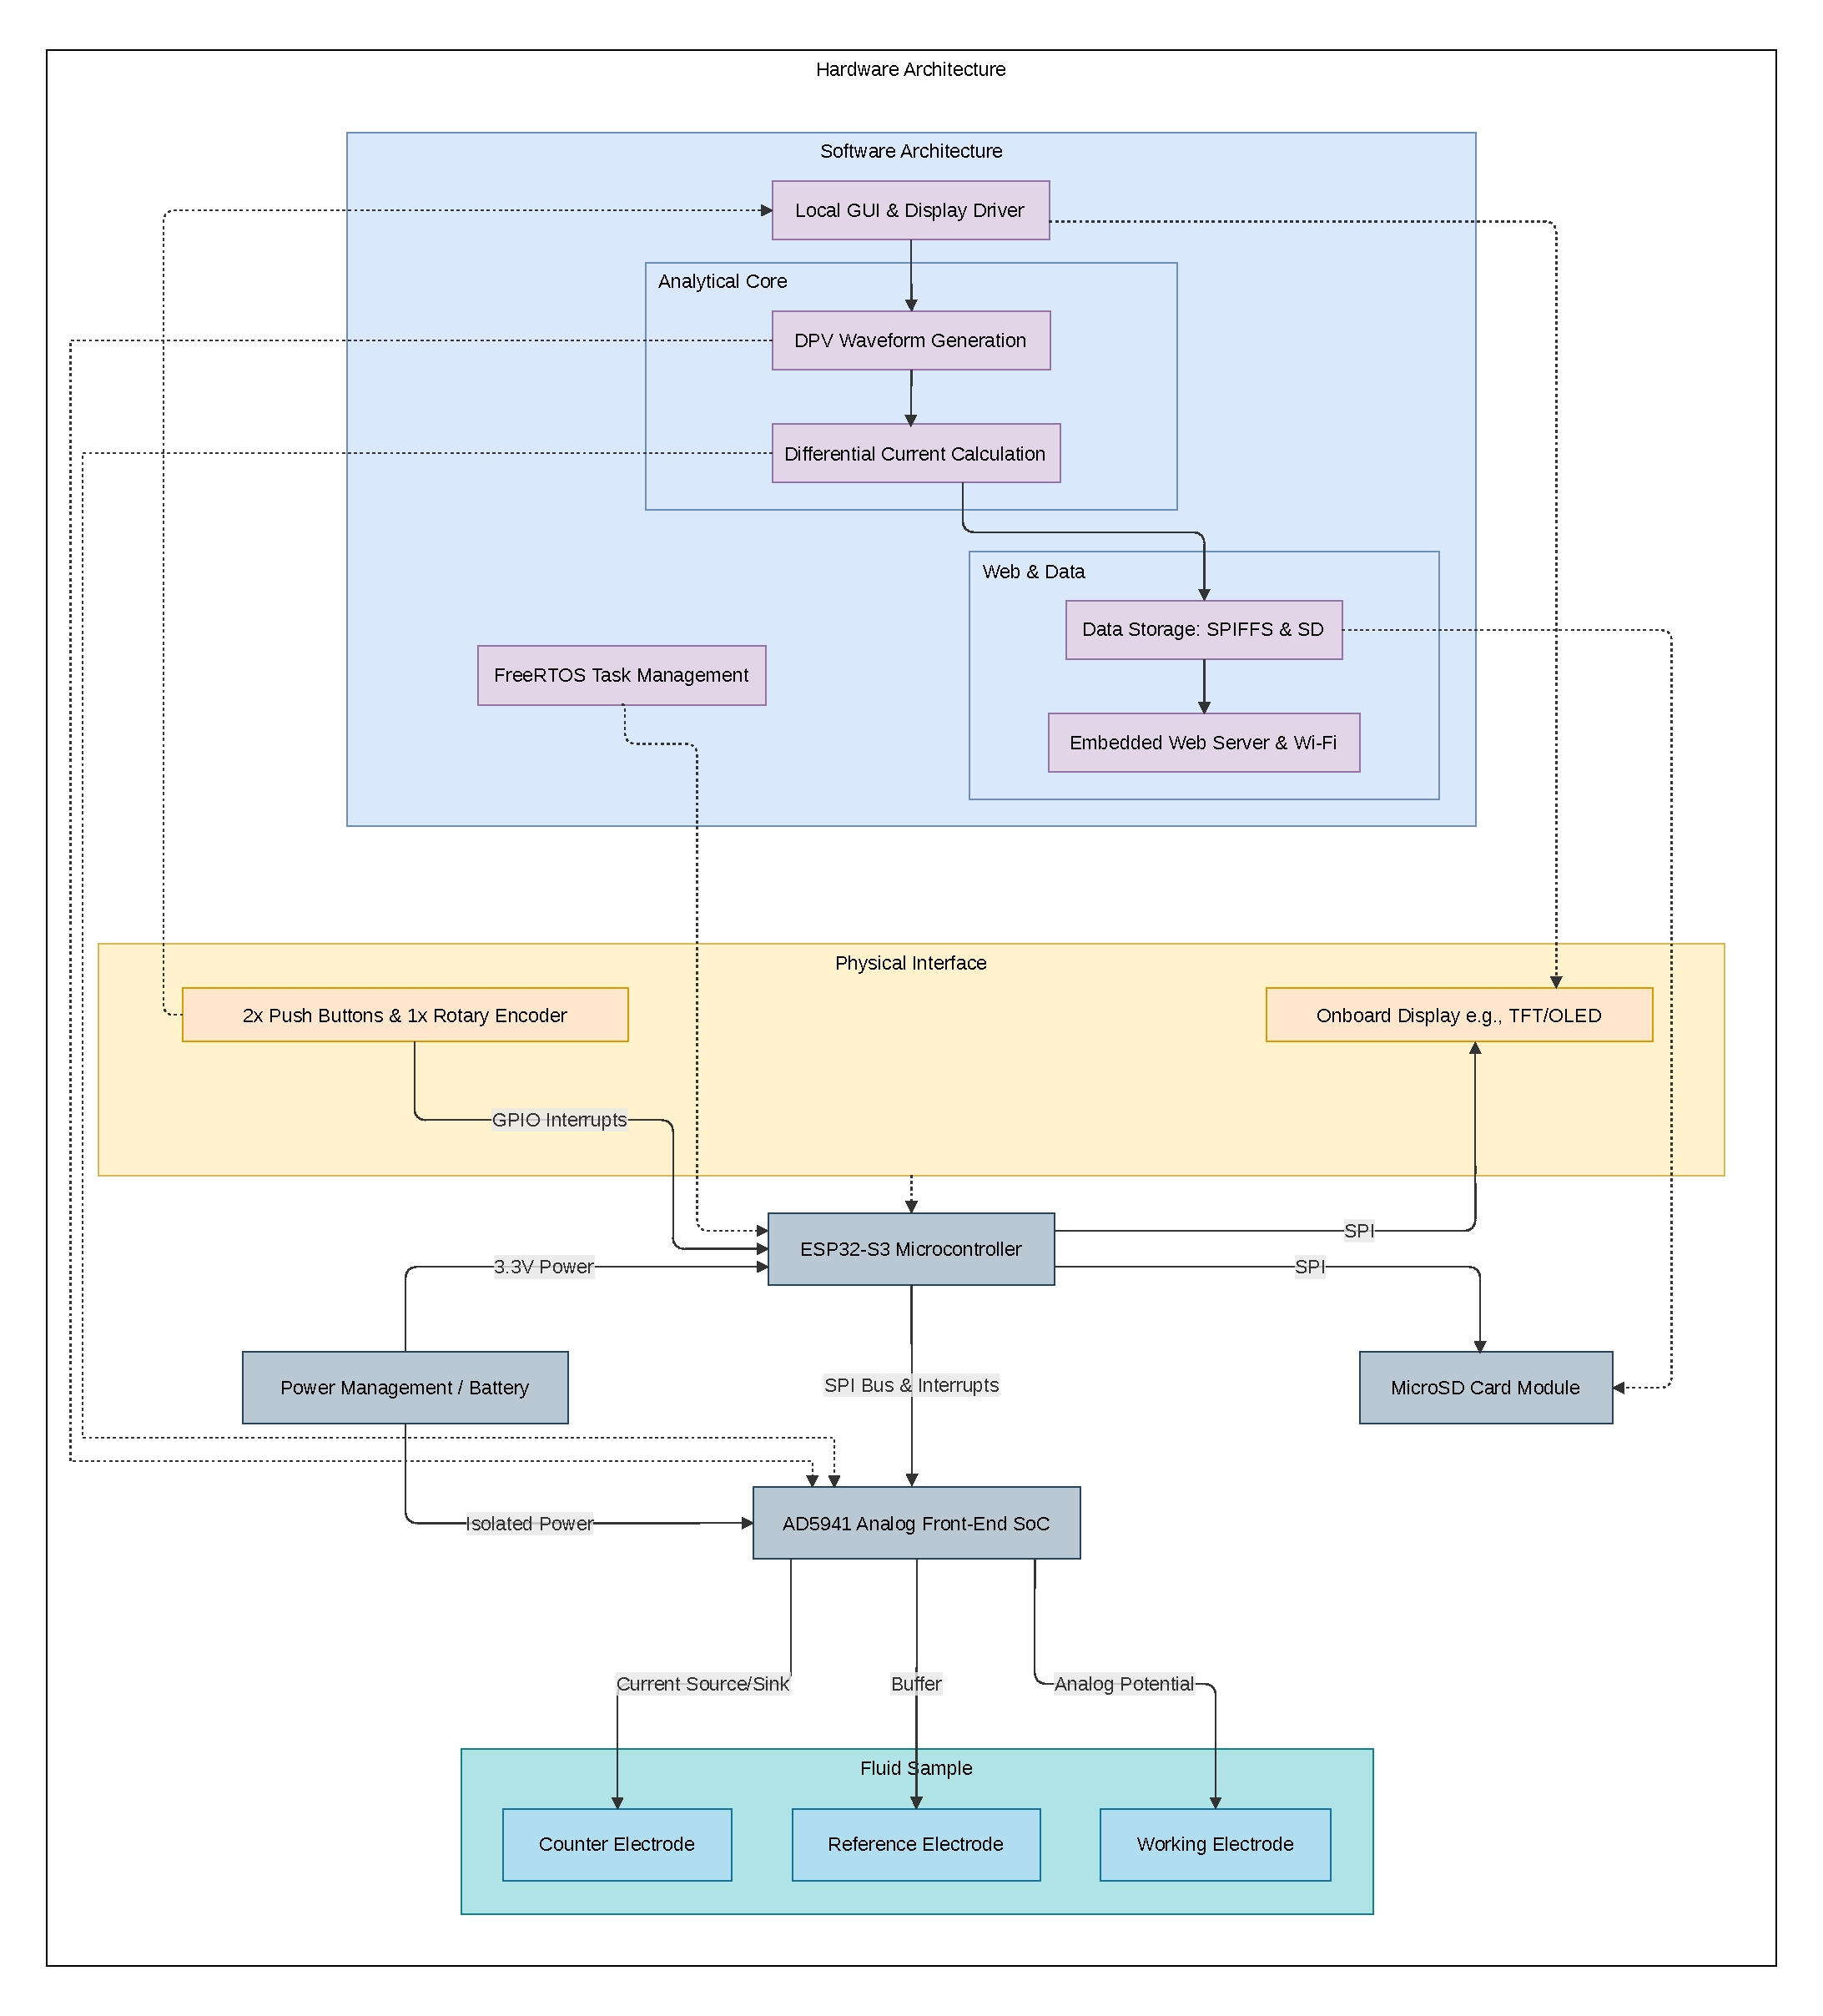
\includegraphics[width=0.9\textwidth]{figures/SystemArchitecture.pdf}
    \caption{System Architecture Diagram}
    \label{fig:system_architecture}
\end{figure}


\section{Electrochemical Cell \& Equivalent Circuit Modeling}
% Focus: Transforming electrochemistry into an electrical model.

% TODO: Model the three-electrode cell using a Randles Equivalent Circuit.
% Discuss solution resistance (R_s), double-layer capacitance (C_{dl}), and charge-transfer resistance (R_{ct}).

It is possible to model the electrochemical cell as a Randle's equivalent circuit, as seen in Figure \ref{fig:randles_circuit}. After defining the system architecture required to interface with the electrochemical cell, it is required to mathematically model what the cell presents to the system. The Randle equivalent circuit is a complex non-ideal impedance model that changes depending on frequency, applied potential and the electrochemical reaction occurring at the working electrode. To design a control loop capable of driving this load reliably, the cell must first be reduced to an equivalent electrical model. A widely used representation of the cell is the Randles equivalent circuit \cite{Laschuk2021}. This equivalent circuit models the electrode and electrolyte interface as a series solution resistance ($R_s$) in series with a parallel combination of the double-layer capacitance ($C_{dl}$) and the charge-transfer resistance ($R_{ct}$). The Warburg impedance ($Z_W$) is included to account for diffusion effects at low frequencies. This model allows for the analysis of the electrochemical cell's behavior under different conditions and is essential for designing the potentiostat's control loop \cite{sannino2025potentiostat}.


% Mathematically derive why pulse voltammetry (like DPV) isolates faradaic analytical current from capacitive charging current based on their exponential decay time constants.

\begin{figure}[H]
    \centering
    \begin{circuitikz}[american, thick]
        % Input from Working Electrode (WE)
        \draw (0,0) node[anchor=east] {WE} to[short, o-] (0.5,0)
        % Solution Resistance (Rs)
        to[R, l=$R_s$] (2.5,0);
        
        % Split into parallel branches
        % Top branch: Double Layer Capacitance (Cdl)
        \draw (2.5,0) -- (2.5,1.5) 
        to[C, l=$C_{dl}$] (6.5,1.5) -- (6.5,0);
        
        % Bottom branch: Charge Transfer Resistance (Rct) and Warburg (Zw)
        \draw (2.5,0) -- (2.5,-1.5) 
        to[R, l=$R_{ct}$] (4.5,-1.5)
        to[generic, l=$Z_W$] (6.5,-1.5) -- (6.5,0);
        
        % Output to Counter/Reference Electrode (CE/RE)
        \draw (6.5,0) to[short, -o] (7,0) node[anchor=west] {CE/RE};
    \end{circuitikz}
    \caption{Randles equivalent circuit modeling the electrochemical cell interface.}
    \label{fig:randles_circuit}
\end{figure}

The link between DPV waveforms and the Randles equivalent circuit is found through identifying the electrical demand it places on the potentiostat. The combination of the $R_s$ and $R_{ct}$ resistors is the total resistive load that must be driven by the control amplifier to sustain the target faradaic current. This resistive load dictates the compliance voltage that the system requires \cite{pineresearch_compliance}. The combination of $R_s$ and $C_{dl}$ form a RC time constant which dictates how quickly the double layer capacitance charges after each step in potential. This time constant governs how long a DPV pulse should be held to ensure that the background current has sufficiently decayed relative to the faradaic current \cite{bard2001}. Rather than being arbitrary selections, parameters such as pulse width, TIA gain, and control-amplifier bandwidth are strictly dictated by the expected $R_s$, $C_{dl}$, and $R_{ct}$ values of the target analyte-electrode interface. If the sampling scheme or amplifier bandwidth fails to match this characteristic RC time constant, the system cannot effectively filter out the unwanted capacitive component of the measured current\cite{sannino2025potentiostat}.

\subsection{Proving Capacitive Current Rejection in DPV}

DPV's effectiveness relies on the different decay rates of the two current components generated at an electrode following a potential step.

\subsubsection{Total Current at the Electrode}

When a potential step is applied, the total measured current is the sum of the faradaic and capacitive components:

\begin{equation}
I_{total}(t) = I_f(t) + I_c(t)
\end{equation}

\begin{table}[htbp]
\centering
\begin{tabular}{l l l l}
\toprule
\textbf{Current Type} & \textbf{Source} & \textbf{Decay Function} & \textbf{Decay Rate} \\
\midrule
Capacitive ($I_c$) & \makecell[l]{Charging the electrical \\ double layer} & $e^{-t/RC}$ & \makecell[l]{Very fast \\ (exponential)} \\
\addlinespace
Faradaic ($I_f$) & \makecell[l]{Electron transfer} & $1/\sqrt{t}$ & \makecell[l]{Slower \\ (inverse square root)} \\
\bottomrule
\end{tabular}
\caption{Comparison of Capacitive and Faradaic Currents}
\label{tab:current_types}
\end{table}

The capacitive current models the electrode-solution interface as an $RC$ circuit, decaying exponentially \cite{palmsens_capacitive_current}:

\begin{equation}
I_c(t) = \frac{\Delta E}{R_s} \, e^{-t/R_sC_{dl}}
\end{equation}

Where: 
\begin{itemize}

\item $R_s$ is the solution resistance.
\item $C_{dl}$ is the double-layer capacitance.
\item $\Delta E$ is the applied potential step.

\end{itemize}

The faradaic current is governed by the Cottrell equation for planar diffusion, decaying with the inverse square root of time \cite{bard2001}:

\begin{equation}
I_f(t) = \frac{nFA\sqrt{D}\,C^*}{\sqrt{\pi t}}
\end{equation}

Where: 

\begin{itemize}
    \item $n$ is the number of electrons transferred.
    \item $F$ is Faraday's constant.
    \item $A$ is the electrode area.
    \item $D$ is the diffusion coefficient.
    \item $C^*$ is the bulk analyte concentration.
\end{itemize}

Because an exponential function ($e^{-t/RC}$) tends toward zero faster than an inverse square root function ($1/\sqrt{t}$), by waiting for a sufficient amount of time after applying the pulse ensures the capacitive current disappeared while the faradaic current remains. 
\subsubsection{The Pulse-Sampling Scheme}

To utilise the property difference between the two current types, DPV applies a series of short voltage pulses superimposed on a linear staircase ramp. To isolate the faradaic current, the potentiostat samples the current twice per pulse cycle:

\begin{enumerate}
    \item $I_{before}$: sampled just before the pulse is applied.
    \item $I_{end}$: sampled at the very end of the pulse duration ($t = \tau_{pulse}$).
\end{enumerate}

\subsubsection{The Differential Proof}

The final output plotted in a DPV voltammogram is the difference between these two samples:

\begin{equation}
\Delta I = I_{end} - I_{before}
\end{equation}

Expanding using the component currents:

\begin{equation}
\Delta I = \left(I_{f,end} + I_{c,end}\right) - \left(I_{f,before} + I_{c,before}\right)
\end{equation}

Finding a solution to the decay mathematics to solve the problem:

\begin{itemize}
    \item Since $I_{before}$ is sampled just before the pulse, the system has been at a baseline potential for a sufficient amount of time so that any previous capacitive transient current has decayed completely. Thus, $I_{c,before} \approx 0$.
    \item Since $I_{end}$ is sampled at the very end of the pulse duration, the new capacitive transient caused by the pulse has also decayed to near zero. Thus, $I_{c,end} \approx 0$.

\end{itemize}

Therefore, the differential in Equation 3.5 simplifies to:

\begin{equation}
\Delta I \approx I_{f,end} - I_{f,before}
\end{equation}

By subtracting $I_{before}$ from $I_{end}$, DPV mathematically rejects the background charging current, leaving only the faradaic signal of interest.

\subsubsection{Why the Output Forms a Peak}

Because $\Delta I$ represents the change in faradaic current for a small, discrete step in potential ($\Delta E$), the resulting plot of $\Delta I$ versus $E$ is effectively an approximation of the derivative of a standard current-potential curve:

\begin{equation}
\Delta I \approx \frac{dI_f}{dE} \cdot \Delta E
\end{equation}

For a reversible system (electron transfer is so fast the system is always in thermodynamic equilibrium) governed by the Nernst equation, taking the derivative of the standard sigmoidal voltammogram produces a Gaussian-like peak. This peak reaches its maximum amplitude exactly at the half-wave potential ($E_{1/2}$), providing an incredibly sensitive and easily quantifiable signal \cite{Laborda2014}.


\section{Analog Front-End Stability \& Control Loop Modeling}
% Focus: Ensuring the potentiostat feedback loop is stable and noise-free.

% TODO: Detail how the double-layer capacitance (C_{dl}) adds a pole to the feedback path, threatening loop stability. 
% Derive the transfer function of the transimpedance amplifier (TIA).

The generalized transfer function for the transimpedance amplifier is defined as:
\begin{equation}
    H(s) = \frac{V_{\text{out}}(s)}{I_{\text{in}}(s)} = - \frac{R_f}{1 + s R_f C_f}
    \label{eq:tia_transfer}
\end{equation}

\subsection{Impact of C\textsubscript{dl} on TIA Loop Stability}

The working electrode connects directly to the summing junction (virtual ground) of the transimpedance amplifier (TIA). Because the double-layer capacitance, $C_{dl}$, physically exists between the working electrode and the bulk solution, it appears electrically as a shunt capacitance from the TIA's inverting input node to ground -- functionally identical to the junction capacitance of a photodiode in a conventional TIA design \cite{graeme1996}. This section derives the TIA transfer function to show how $C_{dl}$ introduces an additional pole into the feedback loop, degrading phase margin and threatening stability.

\subsubsection{Circuit Model and Node Equation}

Let $R_f$ be the TIA feedback resistor, $C_{dl}$ the shunt capacitance at the inverting node, and $A(s)$ the open-loop gain of the operational amplifier. Let $V_n$ be the voltage at the inverting node and $I_{in}$ the faradaic current sourced by the electrochemical reaction. Applying KCL at the summing node:

\begin{equation}
I_{in} = V_n \, sC_{dl} + \frac{V_n - V_{out}}{R_f}
\label{eq:kcl}
\end{equation}

Since the op-amp enforces $V_{out} = -A(s)V_n$ (with the non-inverting input grounded), we have:

\begin{equation}
V_n = -\frac{V_{out}}{A(s)}
\label{eq:vn}
\end{equation}

Substituting Equation~\eqref{eq:vn} into Equation~\eqref{eq:kcl} and solving for $V_{out}/I_{in}$ gives the closed-loop transimpedance:

\begin{equation}
Z_T(s) \equiv \frac{V_{out}}{I_{in}} = \frac{-R_f}{1 + \dfrac{1 + sR_fC_{dl}}{A(s)}}
\label{eq:ZT}
\end{equation}

\subsubsection{Noise Gain and the Loop Gain Pole}

Define the \emph{noise gain} of the feedback network as:

\begin{equation}
NG(s) = 1 + sR_fC_{dl}
\label{eq:NG}
\end{equation}

Equation~\eqref{eq:NG} shows that $C_{dl}$ introduces a \emph{zero} into the noise gain at:

\begin{equation}
f_z = \frac{1}{2\pi R_f C_{dl}}
\label{eq:fz}
\end{equation}

Above $f_z$, the noise gain rises at $+20\,\mathrm{dB/decade}$. The op-amp itself is modelled as a single-dominant-pole system, $A(s) = \omega_t/s$ near the crossover region, where $\omega_t = 2\pi \, \text{GBW}$ is the unity-gain angular frequency. The loop gain is therefore:

\begin{equation}
T(s) = \frac{A(s)}{NG(s)} = \frac{\omega_t}{s(1+sR_fC_{dl})}
\label{eq:loopgain}
\end{equation}

Equation~\eqref{eq:loopgain} reveals the core stability problem: the zero that $C_{dl}$ introduced into the noise gain (Eq.~\eqref{eq:NG}) becomes an additional \emph{pole} in the loop gain, located at:

\begin{equation}
\omega_{p2} = \frac{1}{R_f C_{dl}}
\end{equation}

Combined with the op-amp's intrinsic pole at the origin (from the integrator-like $\omega_t/s$ term), the loop gain $T(s)$ now contains \emph{two} poles below the crossover frequency.

\subsubsection{Phase Margin Degradation}

The closed-loop crossover frequency $\omega_{cl}$, where $|T(j\omega_{cl})| = 1$, is found by setting the magnitude of Equation~\eqref{eq:loopgain} to unity. For $\omega_{cl} \gg 1/(R_fC_{dl})$ (the typical high-bandwidth case):

\begin{equation}
|T(j\omega)| \approx \frac{\omega_t}{\omega^2 R_f C_{dl}} = 1
\quad \Longrightarrow \quad
\omega_{cl} = \sqrt{\frac{\omega_t}{R_f C_{dl}}}
\label{eq:wcl}
\end{equation}

At this crossover frequency, each of the two poles in $T(s)$ contributes close to $-90^\circ$ of phase shift, for a combined phase approaching $-180^\circ$. Since a negative feedback loop becomes unstable once the total loop phase reaches $-180^\circ$ at the frequency where $|T(j\omega)|=1$, the phase margin,

\begin{equation}
\phi_{PM} = 180^\circ - \left|\angle T(j\omega_{cl})\right|,
\end{equation}

collapses toward $0^\circ$. In practice this manifests as pronounced ringing, overshoot, or sustained oscillation in the measured current whenever the electrode's $C_{dl}$ is large relative to $1/(\omega_t R_f)$ -- precisely the condition encountered with high-sensitivity potentiostat designs, where $R_f$ must be large (to resolve nA--pA faradaic currents) and $C_{dl}$ can range from nanofarads to microfarads depending on electrode area and surface roughness \cite{ying2021}.

\subsubsection{Compensation}

Stability is restored by adding a small feedback capacitor $C_f$ in parallel with $R_f$, introducing a compensating pole into the noise gain \emph{before} the $C_{dl}$-induced zero dominates. Choosing $C_f$ such that the noise gain pole occurs at the geometric mean of $f_z$ and the amplifier's gain-bandwidth product restores a single-pole roll-off at crossover, yielding a phase margin close to $45^\circ$--$65^\circ$ \cite{graeme1996}:

\begin{equation}
C_f = \sqrt{\frac{C_{dl}}{2\pi R_f \, \text{GBW}}}
\label{eq:Cf}
\end{equation}

Equation~\eqref{eq:Cf} demonstrates that the compensation capacitor required for stable operation is a direct function of the electrode's double-layer capacitance, reinforcing that the electrochemical cell -- modelled via the Randles equivalent circuit -- is not merely a passive measurement target but an active determinant of the analog front-end's stability margin.

% TODO: Demonstrate how selecting the correct feedback resistor (R_f) and filtering capacitor (C_f) optimizes noise performance and phase margin.

\section{Voltammetric Digital Signal Processing \& Peak Extraction}
% Focus: The direct, deterministic replacement for the Machine Learning section.

% TODO: Map out the classical DSP pipeline. Define the mathematical subtraction formula for DPV.
The differential current is calculated as:
\begin{equation}
    \Delta I = I_{\text{end}} - I_{\text{before}}
    \label{eq:dpv_subtraction}
\end{equation}

% TODO: Detail the digital smoothing model (e.g., a Moving Average or Savitzky-Golay filter). 
% Formulate a derivative-based peak-finding algorithm combined with baseline linear interpolation.

The exact peak potential is automatically isolated by solving for the root of the derivative:
\begin{equation}
    \frac{d(\Delta I)}{dE} = 0
    \label{eq:peak_finding}
\end{equation}

\section{Embedded Communication Protocol \& GUI State Machine}
% Focus: Modeling the software interaction and state-tracking.

% TODO: Define the packet-level SPI communication protocol between the ESP32-S3 and the AD5941 registers.
% Present a formal finite state machine (FSM) or state transition model showing how the system handles asynchronous tasks (managing active scans, physical display refresh, WebSocket streaming) without disrupting ADC timing.

\begin{figure}[H]
    \centering
    % \includegraphics[width=0.8\textwidth]{figures/state_machine.png}
    \caption{Finite state machine diagram for managing asynchronous tasks and WebSocket communication.}
    \label{fig:gui_fsm}
\end{figure}